\documentclass[conference]{IEEEtran}
\IEEEoverridecommandlockouts
\usepackage{cite}
\usepackage{amsmath,amssymb,amsfonts}
\usepackage{algorithmic}
\usepackage{graphicx}
\usepackage{textcomp}
\usepackage{caption} 
\usepackage{hyperref} 
\captionsetup[table]{skip=10pt}
\usepackage{rotating}
\usepackage{makecell}
\usepackage{xcolor}
\def\BibTeX{{\rm B\kern-.05em{\sc i\kern-.025em b}\kern-.08em
    T\kern-.1667em\lower.7ex\hbox{E}\kern-.125emX}}
\begin{document}

\title{Genre-Focused Clustering of Spotify Song Data}

\author{\IEEEauthorblockN{Niki Vasan}
\IEEEauthorblockA{\textit{Quantitative Theory and Methods} \\
\textit{Emory University}\\
Atlanta, GA \\
niki.vasan@emory.edu}
\and
\IEEEauthorblockN{David Gaviria}
\IEEEauthorblockA{\textit{Computer Science} \\
\textit{Emory University}\\
Atlanta, GA \\
dgaviri@emory.edu}
\and
\IEEEauthorblockN{Gianluis Hernandez}
\IEEEauthorblockA{\textit{Computer Science} \\
\textit{Emory University}\\
Atlanta, GA \\
ghern22@emory.edu}}
\maketitle

\thispagestyle{plain}
\pagestyle{plain}

\textbf{Collaboration Statement:} \textit{This project was conducted by the three co-authors of this paper, with consultation by our TA Hope Mumme. No outside sources or peers were consulted outside of relevant documentation.}\newline{}

\begin{abstract}
 This paper uses pre-scraped Spotify song data and unsupervised clustering models to understand how quantitative measures of musicality (e.g. tempo, danceability, instrumentalness) correlate to the genre profile of a song or group of songs, with the broader goal of deriving song recommendations from "similar" songs. Instead of simply using the genre label of a song (e.g. pop, jazz, rap) to suggest similar music, we feed these non-genre attributes into K-Means and DB-Scan clustering algorithms. From there, we attempt to derive clusters of similar songs and compare their genre profiles to see which genres may be listened together frequently. However, we find that this dataset is not well-differentiated via our implementation of these clustering algorithms, with DB-Scan performing marginally better than K-Means. Future research should try different optimizations or density-based clustering models, account for overlap within genre-labels, as well as ensuring a broader and more representative sample of songs. 
 
\end{abstract}

\section{Problem Description}
A common problem faced by those who enjoy listening to music is finding songs similar to those they already like. While this can be done based off word-of mouth, it is more efficient to employ algorithms that harness the power of big databases. However, designing such an algorithm evokes several challenges. The first is that modern musical databases often contain millions of songs, which makes exhaustively searching for similar songs an infeasible task. The second is that while many songs are already categorized by genre, these labels may be manually assigned and are thus prone to error or overlap with existing typologies. Genres are also growing increasingly broad as music evolves (e.g. distinctions between "new wave" RnB versus older RnB), motivating the need to consider other attributes of a song to create a more personalized user experience.

Thus, in this project, we explore ways of finding similar songs without relying on genre categorization. We propose using clustering methods, specifically K-Means and DB-Scan, to place songs into clusters based on similarity among a set of features. We anticipate two main applications of this work: 1) once the clusters are created, we can back-reference the original genre labels to their respective samples and discover the 'genre composition' of each cluster (e.g. understand what genres are frequently listened together) 2) future work can then run an algorithm such as KNN to efficiently find similar songs to a given input, preventing the need for conducting computationally expensive searches on large databases. In this manner, we will be able to better understand differentiation between genre labels while also building the foundation for recommending songs based on quantitative measures of musicality.   

\section{Data Description}

The data used was the \href{https://www.kaggle.com/datasets/mrmorj/dataset-of-songs-in-spotify?resource=download} {genres dataset} from Kaggle.  This dataset is pre-scraped data from Spotify's API and is composed of 22 attributes with over 42,000 samples. There are several attributes that are specific to the API call (e.g. urls) or do not relate to the musical characteristics of the song itself (e.g. IDs, duration), so we ignore those. Instead, we look at the following 10 attributes:

    \begin{enumerate}
        \item Danceability
        \item Energy
        \item Key
        \item Mode
        \item Speechiness
        \item Acousticness
        \item Instrumentalness
        \item Liveness
        \item Valence
        \item Tempo
    \end{enumerate}

We also keep the genre attribute, which states the genre of the song according to Spotify's internal genre classification system. This attribute is not used in clustering the data, but is attached to the samples afterwards to assess the 'genre profiles' of each cluster.

\section{Data Pre-processing}
Pre-processing the data is prerequisite to implementing any data mining technique. The data must be cleaned and features must be selected and scaled appropriately to ensure strong model performance. In this section, we describe the initial steps taken to pre-process this dataset. Note that after implementing the models and discovering their ineffectiveness at clustering the data, we revisit the feature selection step, utilizing scatterplots to assess the clustering tendency of the data and selecting different subsets of the data to assess any changes in performance. 

\subsection{Data Cleaning} 
First, we check if any of the features have missing values or anomalies. We discover that around 50\% of the records have a missing song name, which could be problematic if we needed to access the names of similar songs. However, the original data had two other attributes, 'title' and 'Unnamed.' We filled in the missing values in 'song\_name' with available values in either of the above attributes. This resulted in only 6 records that had no available song name across the three attributes. These records were dropped, along with the columns unrelated to our project. 

\subsection{Feature Selection}
The next step is to select the features that will be used in the clustering. After dropping irrelevant features, there are only 11 features left. For a dataset with roughly 42k entries, this doesn't make the dataset significantly high dimensional. Still, to mitigate potential collinearity among features and because all the features are numeric, we use a Pearson Correlation Matrix. 

\begin{figure}[!ht]
    \begin{center}
        \resizebox{\columnwidth}{!}{
            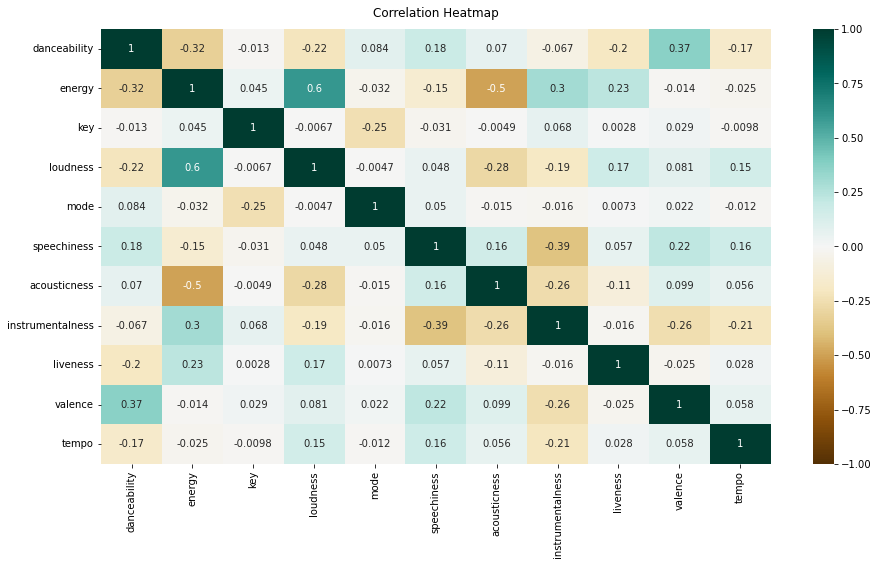
\includegraphics[width=\textwidth]{pearson-matrix.png}
        }
    \end{center}
    \caption{Pearson Correlation Matrix}
    \label{fig:corr_matrix}
\end{figure}

From Figure \ref{fig:corr_matrix}, we can observe an inverse relationship between 'acousticness' and 'energy' (corr = -0.5). There also appears to be a positive relationship between loudness and energy (corr = 0.6). This relationship is better visualized in the following scatterplot. 

\begin{figure}[!ht]
    \begin{center}
        \resizebox{\columnwidth}{!}{
            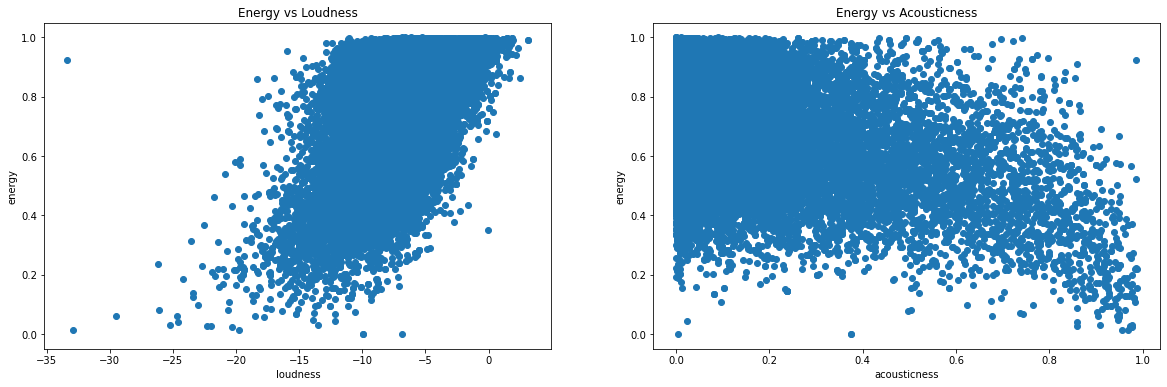
\includegraphics[width=\textwidth]{energy-scatter.png}
        }
    \end{center}
    \caption{Genre-Feature Relationships}
    \label{fig:corr-scatter}
\end{figure}

Energy appears to be correlated to other features, however we can see from Figure \ref{fig:feature-genre-corr} that it also is the attribute with the strongest correlation to the 'genre' label Spotify assigns to a song. This makes us hesitant to remove it from the model, as it is clear the metric is significant in terms of quantifying song similarity. Instead, we choose to remove loudness, which has the highest correlation to energy out of all attributes.

\begin{figure}[!ht]
    \begin{center}
        \resizebox{\columnwidth}{!}{
            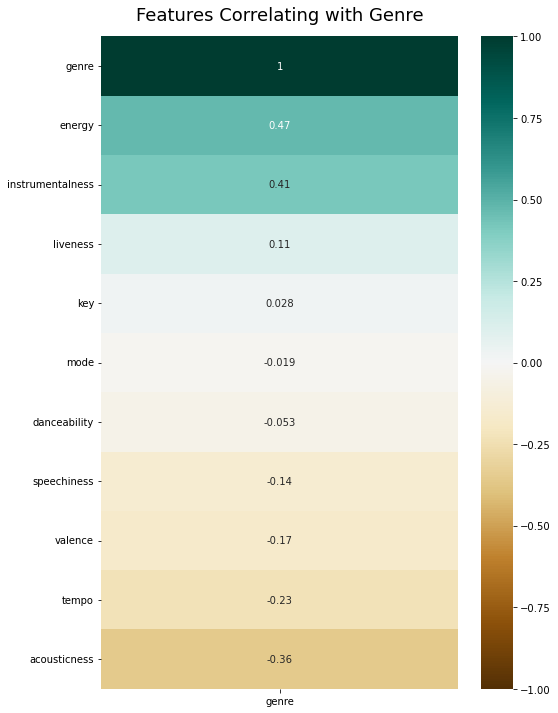
\includegraphics[width=\textwidth]{feature-genre-corr.png}
        }
    \end{center}
    \caption{Genre-Feature Relationships}
    \label{fig:feature-genre-corr}
\end{figure}

\subsection{Feature Scaling}
The last step of the initial pre-processing phase is normalizing the dataset. A quick call to the `describe()` function in pandas illustrates that each of the features, although all numeric, operate on different scales. Since we are using clustering algorithms that use Euclidean distance metrics, they will be sensitive to feature scale. We chose to scale the data using z-score normalization, as implemented through `sklearn`'s Standard Scaler class. We left genre, which is a categorical feature, unencoded and unscaled, as it will not be used as a model input but rather a reference. The final dataset contains the normalized attributes listed above, along with genre. 


\section{Data Mining Methods}
 To implement the clustering algorithms, we used the KMeans and DBScan classes from the Scikit-Learn library. A more detailed discussion of their workings can be found below. To facilitate interoperability, the algorithms and parameter tuning were wrapped up in a self-designed ‘GenreClusterer’ class. The parameter 'model type' set the internal model of the class to the desired algorithm.  

 The `main.py` file can be run to process the data, run the algorithms, receive the cluster profile outputs and generate PCA visualizations of each algorithm. The code is designed to be manually adjusted to run different algorithms, parameters or subsets of the data.

\subsection{Train-Test-Split}
First, the data was split into a training and validation set (70-30). We chose not to include a test set, as we were treating both algorithms as unsupervised, meaning there are no ground truth labels for each record. The training set was used to train the actual model, while the validation set was used to determine the optimal hyperparameters, which differ per model. Note, future iterations of this work that build out an additional recommender system may want to set aside some data (~10\%) as testing inputs.

\subsection{Hyperparameter Tuning}
The validation set was then passed to the GenreClusterer, which contains a method called `fit\_parameters` that performed a grid search using 5 fold cross validation to find the optimal parameters for the specified model. These parameters are model-specific. For K-Means, we were searching for the optimal K. For DB-Scan, we were searching for the optimal Epsilon, or maximum radius of the neighborhood of a core point. DB-Scan also has another parameter that can be manipulated, MinPts, but the ClustEval grid search implementation did not including optimizing this parameter. We later implemented a manual grid search that found both the optimal MinPts and Epsilon parameters, resolving the issue. Once the optimal parameters were returned, the training data was then passed to the GenreClusterer, which returned an array of cluster ids, where each id corresponded to the sample in the same array position in the training data.

\subsection{Cluster Profiles}
To analyze the genre composition of each cluster, the GenreClusterer class also implemented a ‘generateClusterProfiles’ method. This method iterates through each cluster's samples and counted the different genres and how many points of the cluster belonged to each. The results were then stored in a list containing [genre, percentage] tuples. 

\subsection{Visualizing Clusters}
Visualizing clusters can be difficult in high-dimensional data, given that plots are most easily interpretable in 2D. To address this issue, the `plot\_components` function visualized the output clusters using Principal Component Analysis. The training data was first fit using sklearn's PCA module. Then, we selected the first two components as the X and Y axes of our plot. We were not concerned with the cumulative explained variance ratio, or how much of the variance in the data is explained by just these two components, because we were not passing in this data to the model. Rather, we were simply using it to configure a plot. Because the cluster "labels" were stored in the model itself, we were able to color the scatterplot according to those labels and return a plot of the data compressed to 2 dimensions.


\section{Results}
The results from this initial study are sub-optimal. Nevertheless, they lend valuable insights as to what improvements should be considered in future iterations of this work. 

Our experiment was conducted in two parts. In Run 1, we use the full training data and in Run 2 we use a small, pre-selected subset of the training data. Performance can be compared across both runs.  

\subsection{Evaluation Metrics}
Because we are utilizing unsupervised clustering techniques, we do not have a ground truth measure to compare our clusters against. There are many ways to assess "goodness-of-clustering" in unsupervised learning problems, but in general, it is important to measure both cluster separation and cluster compactness. Meaningful clusters are those that maximize intra-class similarity and minimize inter-class similarity; in essence, the objects in a cluster are similar to those within their cluster but different to those in other clusters. To assess both these components using one metric, we use the Silhouette Coefficient. This value ranges from -1 to 1, with values of 1 indicating that the cluster is both compact and spatially distinct from other clusters. The higher the Silhouette Coefficient, the better.

\subsection{Run 1: Full Training Data}
\subsubsection{K-Means}
The first clustering algorithm we try is K-Means. This is a simple partitioning-based algorithm that partitions the training data into a set of k clusters identified by k centroids. We find that K-Means performs extremely poorly on our dataset. 

Figure \ref{fig:kmeans-elbow} demonstrates that the optimal k is 2 clusters. After fitting the model using the training data with k=2, we achieve a silhouette coefficient of only 0.1173. We can visualize the relationship between the cluster labels and silhouette value through Figure \ref{fig:kmeans-sil-viz}. 

\begin{figure}[!ht]
    \begin{center}
        \resizebox{\columnwidth}{!}{
            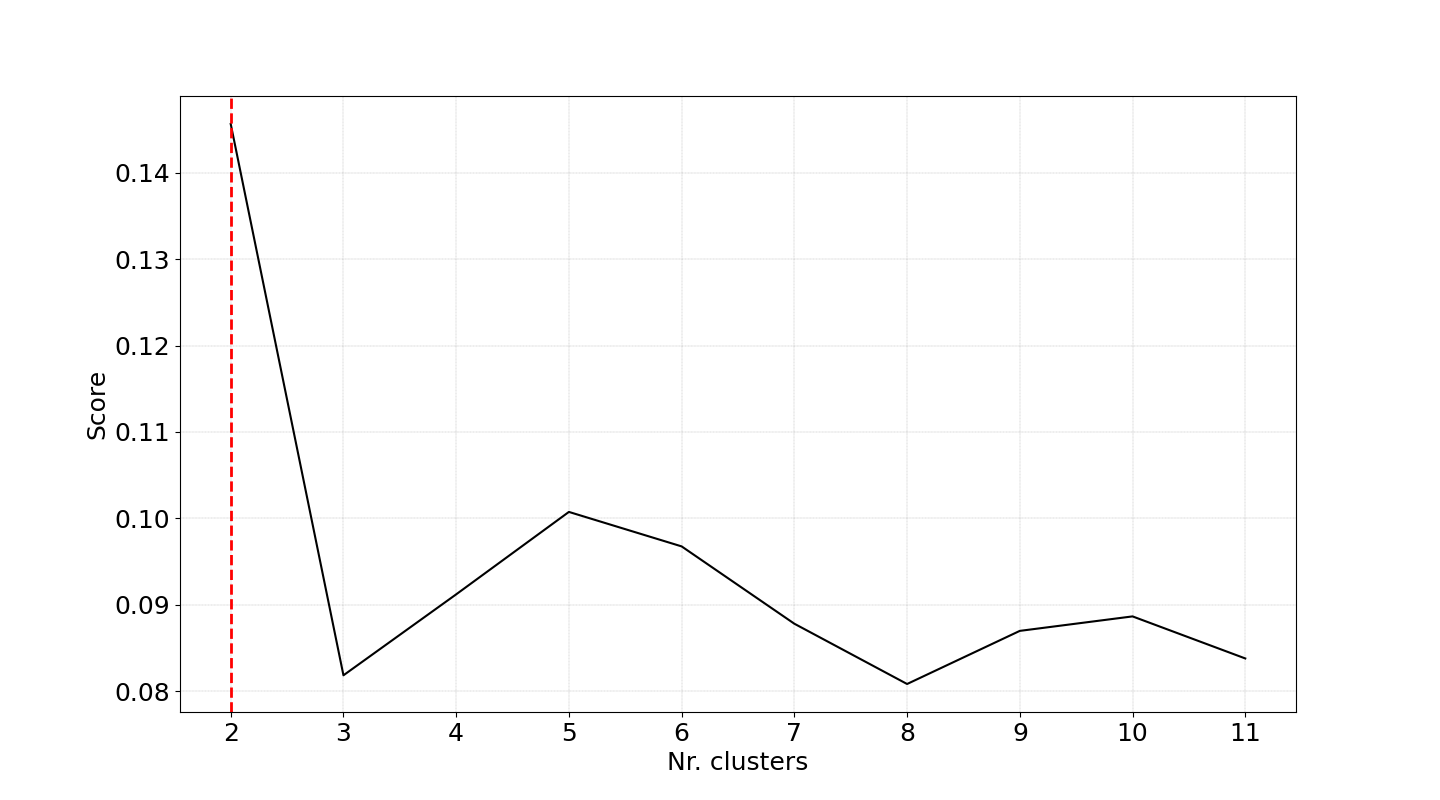
\includegraphics[width=\textwidth]{kmeans-r1.png}
        }
    \end{center}
    \caption{K-Means: Optimal K}
    \label{fig:kmeans-elbow}
\end{figure}

\begin{figure}[!ht]
    \begin{center}
        \resizebox{\columnwidth}{!}{
            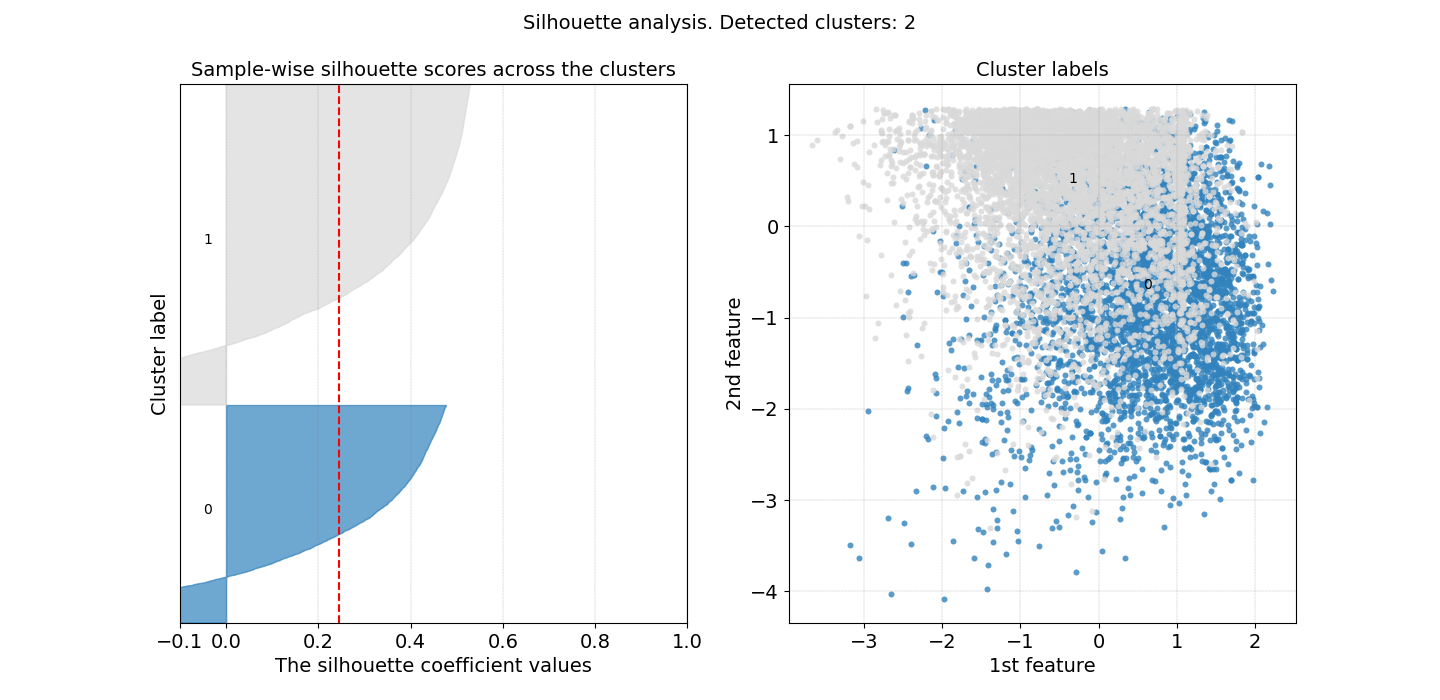
\includegraphics[width=\textwidth]{kmeans-sil-r1.png}
        }
    \end{center}
    \caption{K-Means: Optimal K}
    \label{fig:kmeans-sil-viz}
\end{figure}

The genre composition of the clusters can be see in the Table below. 


\section*{K-MEANS: Genre Composition by Cluster}
\begin{table}[ht!]
    \centering
        \begin{tabular}{| c | c |}
        \hline
        Cluster & Genre Composition \\
        \hline
        Cluster 1 & \makecell{ ('Underground Rap', 0.1534) \\ ('other', 0.1438) \\ ('Dark Trap', 0.1051) \\ ('psytrance', 0.0766) \\ ('trap', 0.0766) \\ ('techhouse', 0.0751) \\ ('techno', 0.0741) \\ ('Hiphop', 0.0685) \\ ('trance', 0.0588) \\ ('Trap Metal', 0.0585) \\ ('dnb', 0.0576) \\ ('Emo', 0.0514) \\ } \\ 
        \hline
        Cluster 2 & \makecell{('Dark Trap', 0.2514) \\ ('Underground Rap', 0.2222) \\ ('Hiphop', 0.15204) \\ ('Trap Metal', 0.1403) \\ ('other', 0.1286) \\ ('Rap', 0.1052) \\ } \\ 
        \hline
        \end{tabular} \\
        \label{tab:kmeans-clust-prof}
\end{table}

% \begin{figure}[!ht]
%     \begin{center}
%         \resizebox{\columnwidth}{!}{
%             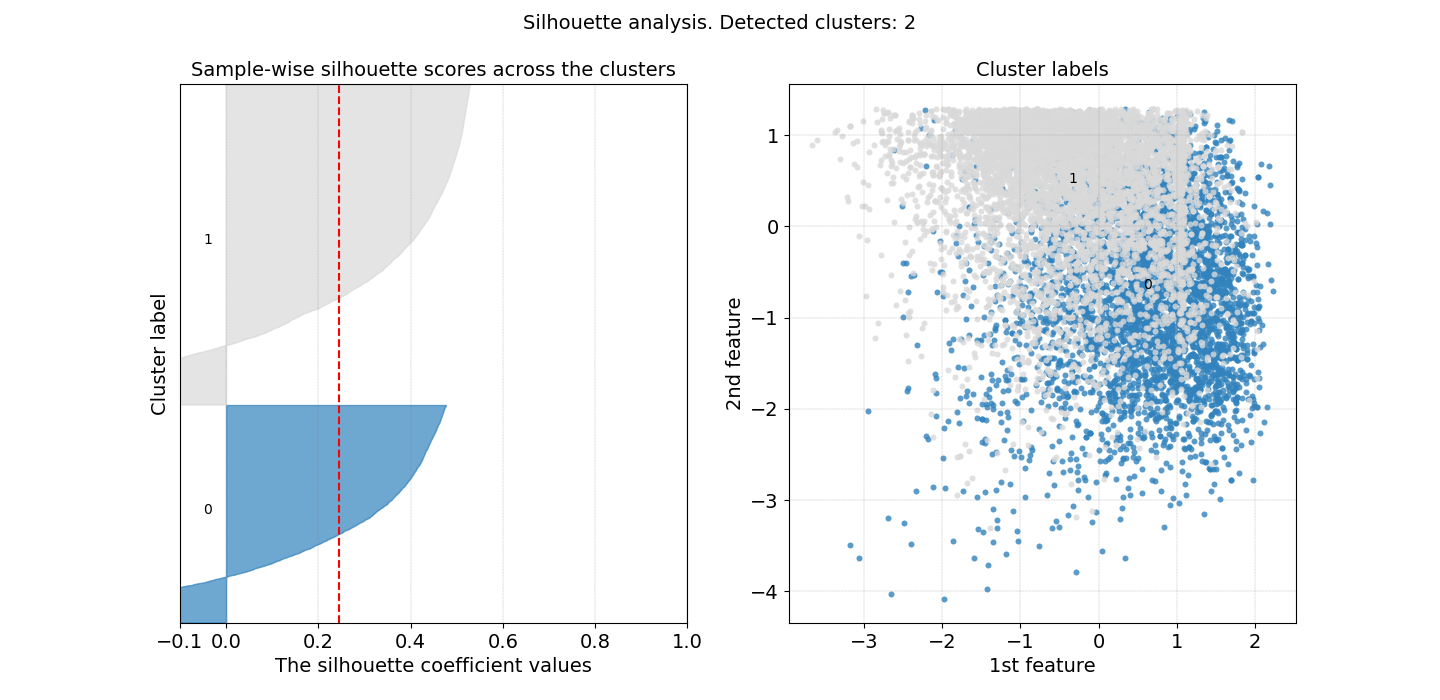
\includegraphics[width=\textwidth]{kmeans-sil-r1.png}
%         }
%     \end{center}
%     \caption{K-Means: Optimal K}
%     \label{fig:kmeans-sil-viz}
% \end{figure}

Cluster 2's results are fairly intuitive and align with a genre-based similarity approach that is commonly used in many music recommendation systems. This cluster is almost entirely composed of genres related to Hiphop/Rap. However, Cluster 1 is interesting because it contains a diverse array of genres, including some found in Cluster 2. Ultimately though, because the silhouette coefficient is so low, we can't say that these results are accurate at this point in time. 

In Figure \ref{fig:kmeans-sil-viz}, we can see that due to the volume and nature of the data (particularly with respect to genre overlap), a connectivity-based clustering approach might prove more fruitful. For this reason, we turn to DB-Scan as our second technique. 

\subsubsection{DB-Scan}
DB-Scan is a density-based clustering technique that can discover clusters of arbitrary shape in high dimensional data. The model requires two parameters: Epsilon and MinPts. As noted before, the clusteval package does not provide a way to search for the optimal MinPts. It does, however, find the optimal Epsilon in relation to the number of clusters and Silhouette Coefficient. Figure \ref{fig:dbscan-eps} is a double line plot generated by clusteval that demonstrates the above relationship. We can see that this graph is extremely choppy, which is already an indication of sub-optimal performance. 

 \begin{figure}[!ht]
    \begin{center}
        \resizebox{\columnwidth}{!}{
            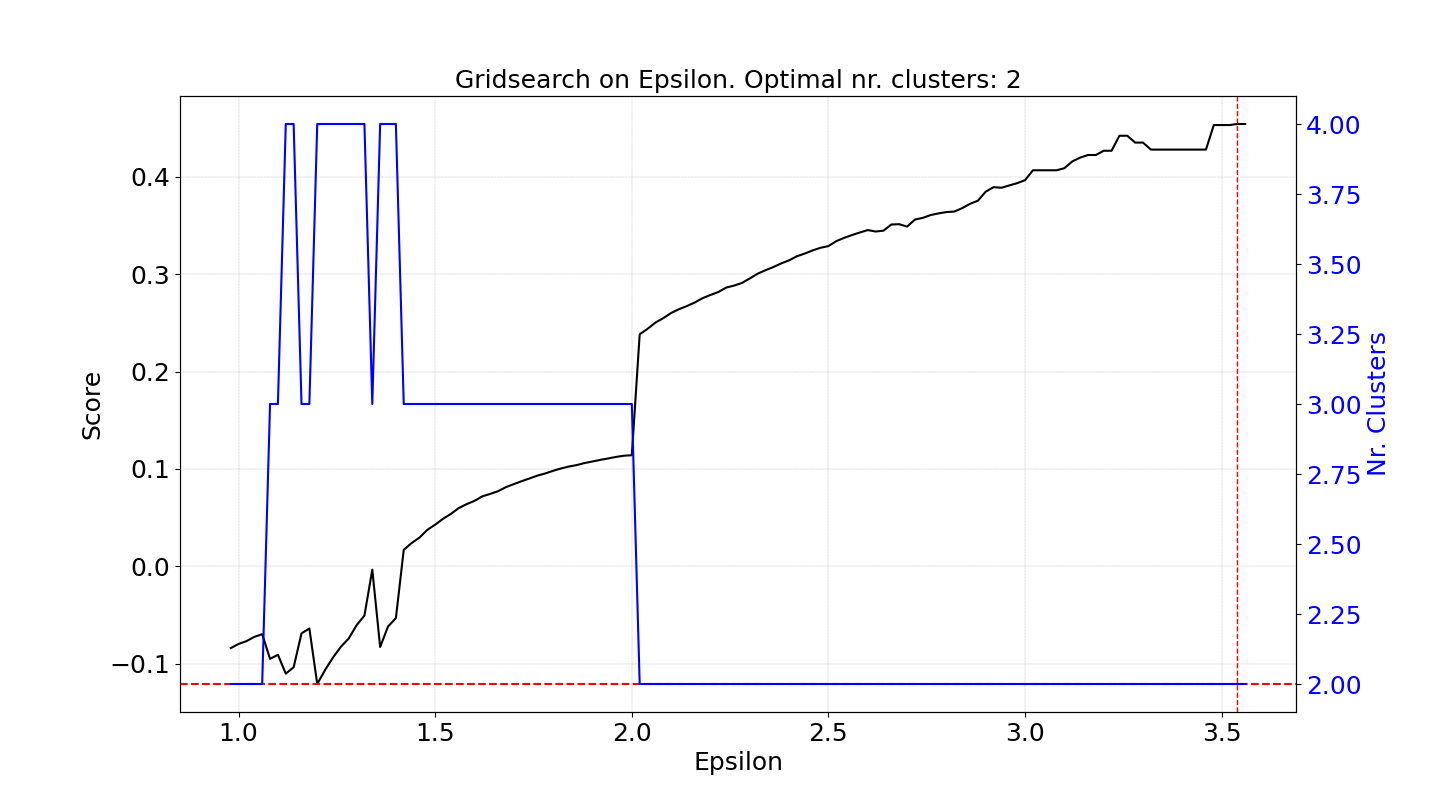
\includegraphics[width=\textwidth]{dbscan-eps-r1.png}
        }
    \end{center}
    \caption{DB-Scan: Optimal Eps}
    \label{fig:dbscan-eps}
\end{figure}


The clusteval package finds the optimal Epsilon to be 3.54 and the associated Silhouette Coefficient on our training set to be 0.454. Our manual grid search implementation finds the optimal parameters as Epsilon = 4.0, MinPts = 3.0, with an associated Silhouette Coefficient of 0.5. This is a negligible improvement. 

Furthermore, even though DB-Scan returns the optimal number of clusters as 2, the model is actually categorizing the entire training set as one cluster and any outliers as another cluster, as shown in Figure \ref{fig:dbscan-pca-r1}. 

 \begin{figure}[!ht]
    \begin{center}
        \resizebox{\columnwidth}{!}{
            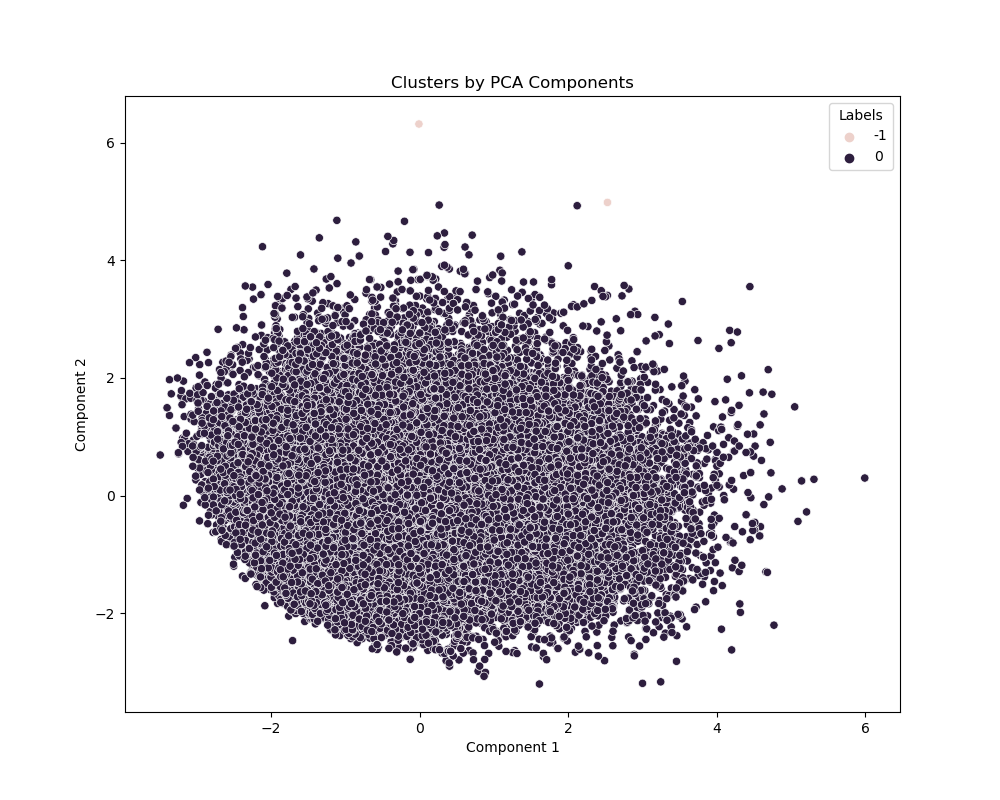
\includegraphics[width=\textwidth]{dbscan-pca-r1.png}
        }
    \end{center}
    \caption{DB-Scan: PCA Cluster Plot}
    \label{fig:dbscan-pca-r1}
\end{figure}

In general, this means the model performs pretty poorly on the full training set. The following table illustrates the cluster profile results for DB-Scan.  

\section*{DB-Scan: Genre Composition by Cluster}
\begin{table}[ht!]
    \centering
        \begin{tabular}{| c | c |}
        \hline
        Cluster & Genre Composition \\
        \hline
        Cluster 1 & \makecell{ ('other', 0.19027191352812023 \\ ('Underground Rap', 0.14004391150143558) \\ ('Dark Trap', 0.10690761695659518) \\ ('psytrance', 0.07150819118392164) \\ ('trance', 0.07103529809153859) \\ ('Hiphop', 0.07086640770140179) \\ ('trap', 0.07046107076507346) \\ ('techhouse', 0.0704272926870461) \\ ('hardstyle', 0.06978550920452627) \\ ('dnb', 0.06938017226819794) \\ ('techno', 0.06931261611214322) } \\ 
        \hline
        Cluster 2 & \makecell{('Trap Metal', 0.75), ('Underground Rap', 0.25), ('other', 0)} \\ 
        \hline
        \end{tabular} \\
        \label{tab:dbscan-clust-prof}
\end{table}

\begin{figure}[!ht]
    \begin{center}
        \resizebox{\columnwidth}{!}{
            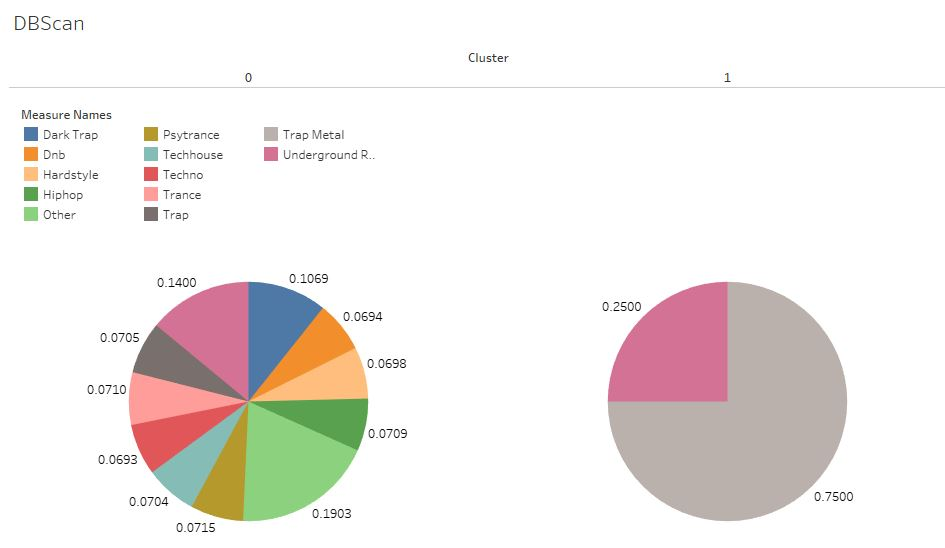
\includegraphics[width=\textwidth]{DBScan Combined.jpg}
        }
    \end{center}
    \caption{Percentage of genres present in each DBScan Cluster}
    \label{fig:clustering-tendency}
\end{figure}


\subsection{Run 2: Subsetted Data}

\subsubsection{Pairwise Analysis}
After receiving the above results, we decide to reduce both the dimensionality and volume of the dataset by focusing on attributes that naturally separate the data and genres that are frequent or do not overlap. To visualize these relationships, we create pairwise scatterplots amongst all the attributes in the data, coloring the data by genre. 

Figure \ref{fig:pairwise-top-5} illustrates all pairwise relationships in the data, filtered by only the top 5 most frequently appearing genres. While we can see some differentiation amongst the genres in certain attribute combinations, given the labels are not fuzzy, we would ideally want more separation. One reason for why the graph may look like this is because the top 5 most frequently occurring genres in the data are: Dark Trap, Underground Rap, Trap Metal, Emo and Rap, most of which are hiphop related genres. 

To test this theory, we further reduce the genres to only Rap and RnB, two musical categories that are generally very different in tempo, style, pace etc. Figure \ref{fig:pairwise-2} illustrates these relationships. We can see that these two genres are best isolated using the attributes 'tempo' and 'liveness.' 

 \begin{figure}[!ht]
    \begin{center}
        \resizebox{\columnwidth}{!}{
            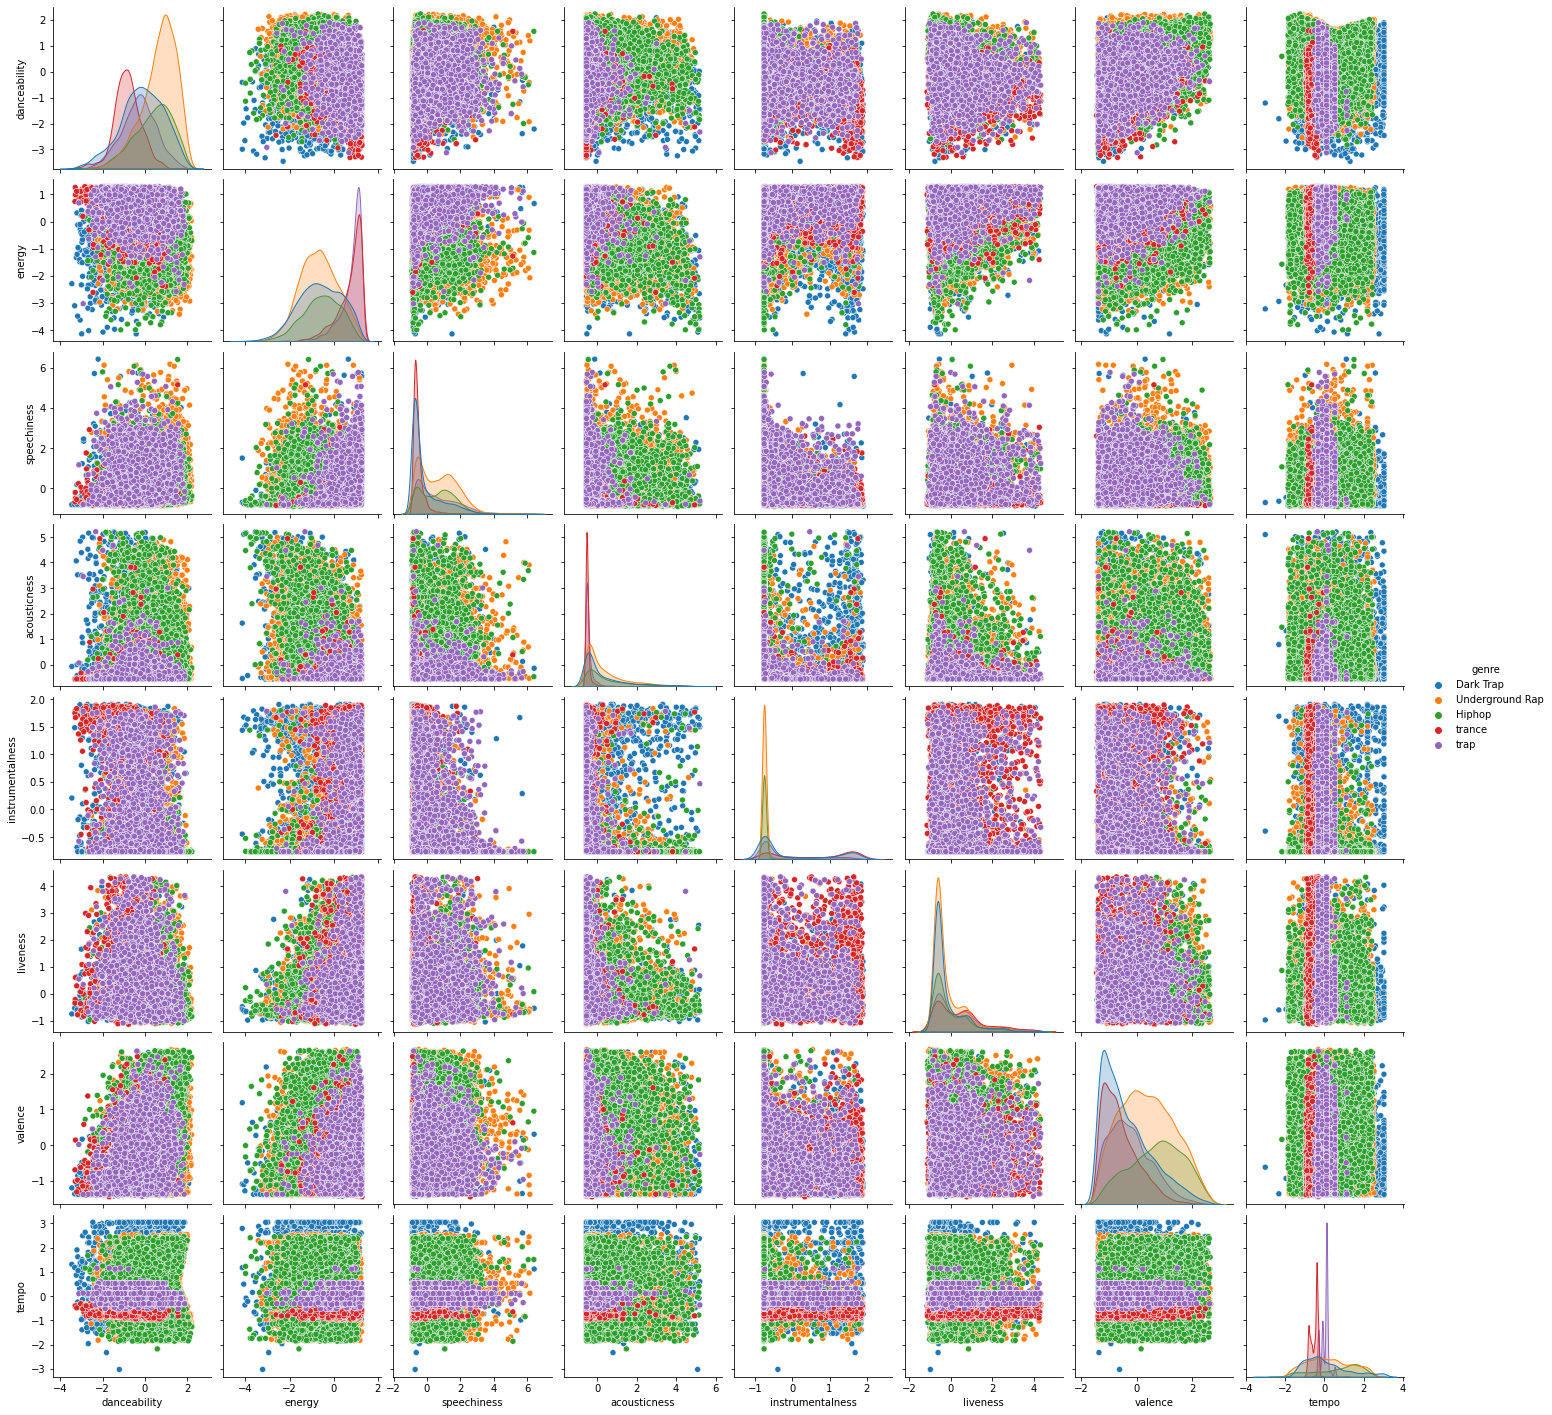
\includegraphics[width=\textwidth]{pairwise-top-5.png}
        }
    \end{center}
    \caption{Pairwise Scatter Plot: Top 5 Genres}
    \label{fig:pairwise-top-5}
\end{figure}


 \begin{figure}[!ht]
    \begin{center}
        \resizebox{\columnwidth}{!}{
            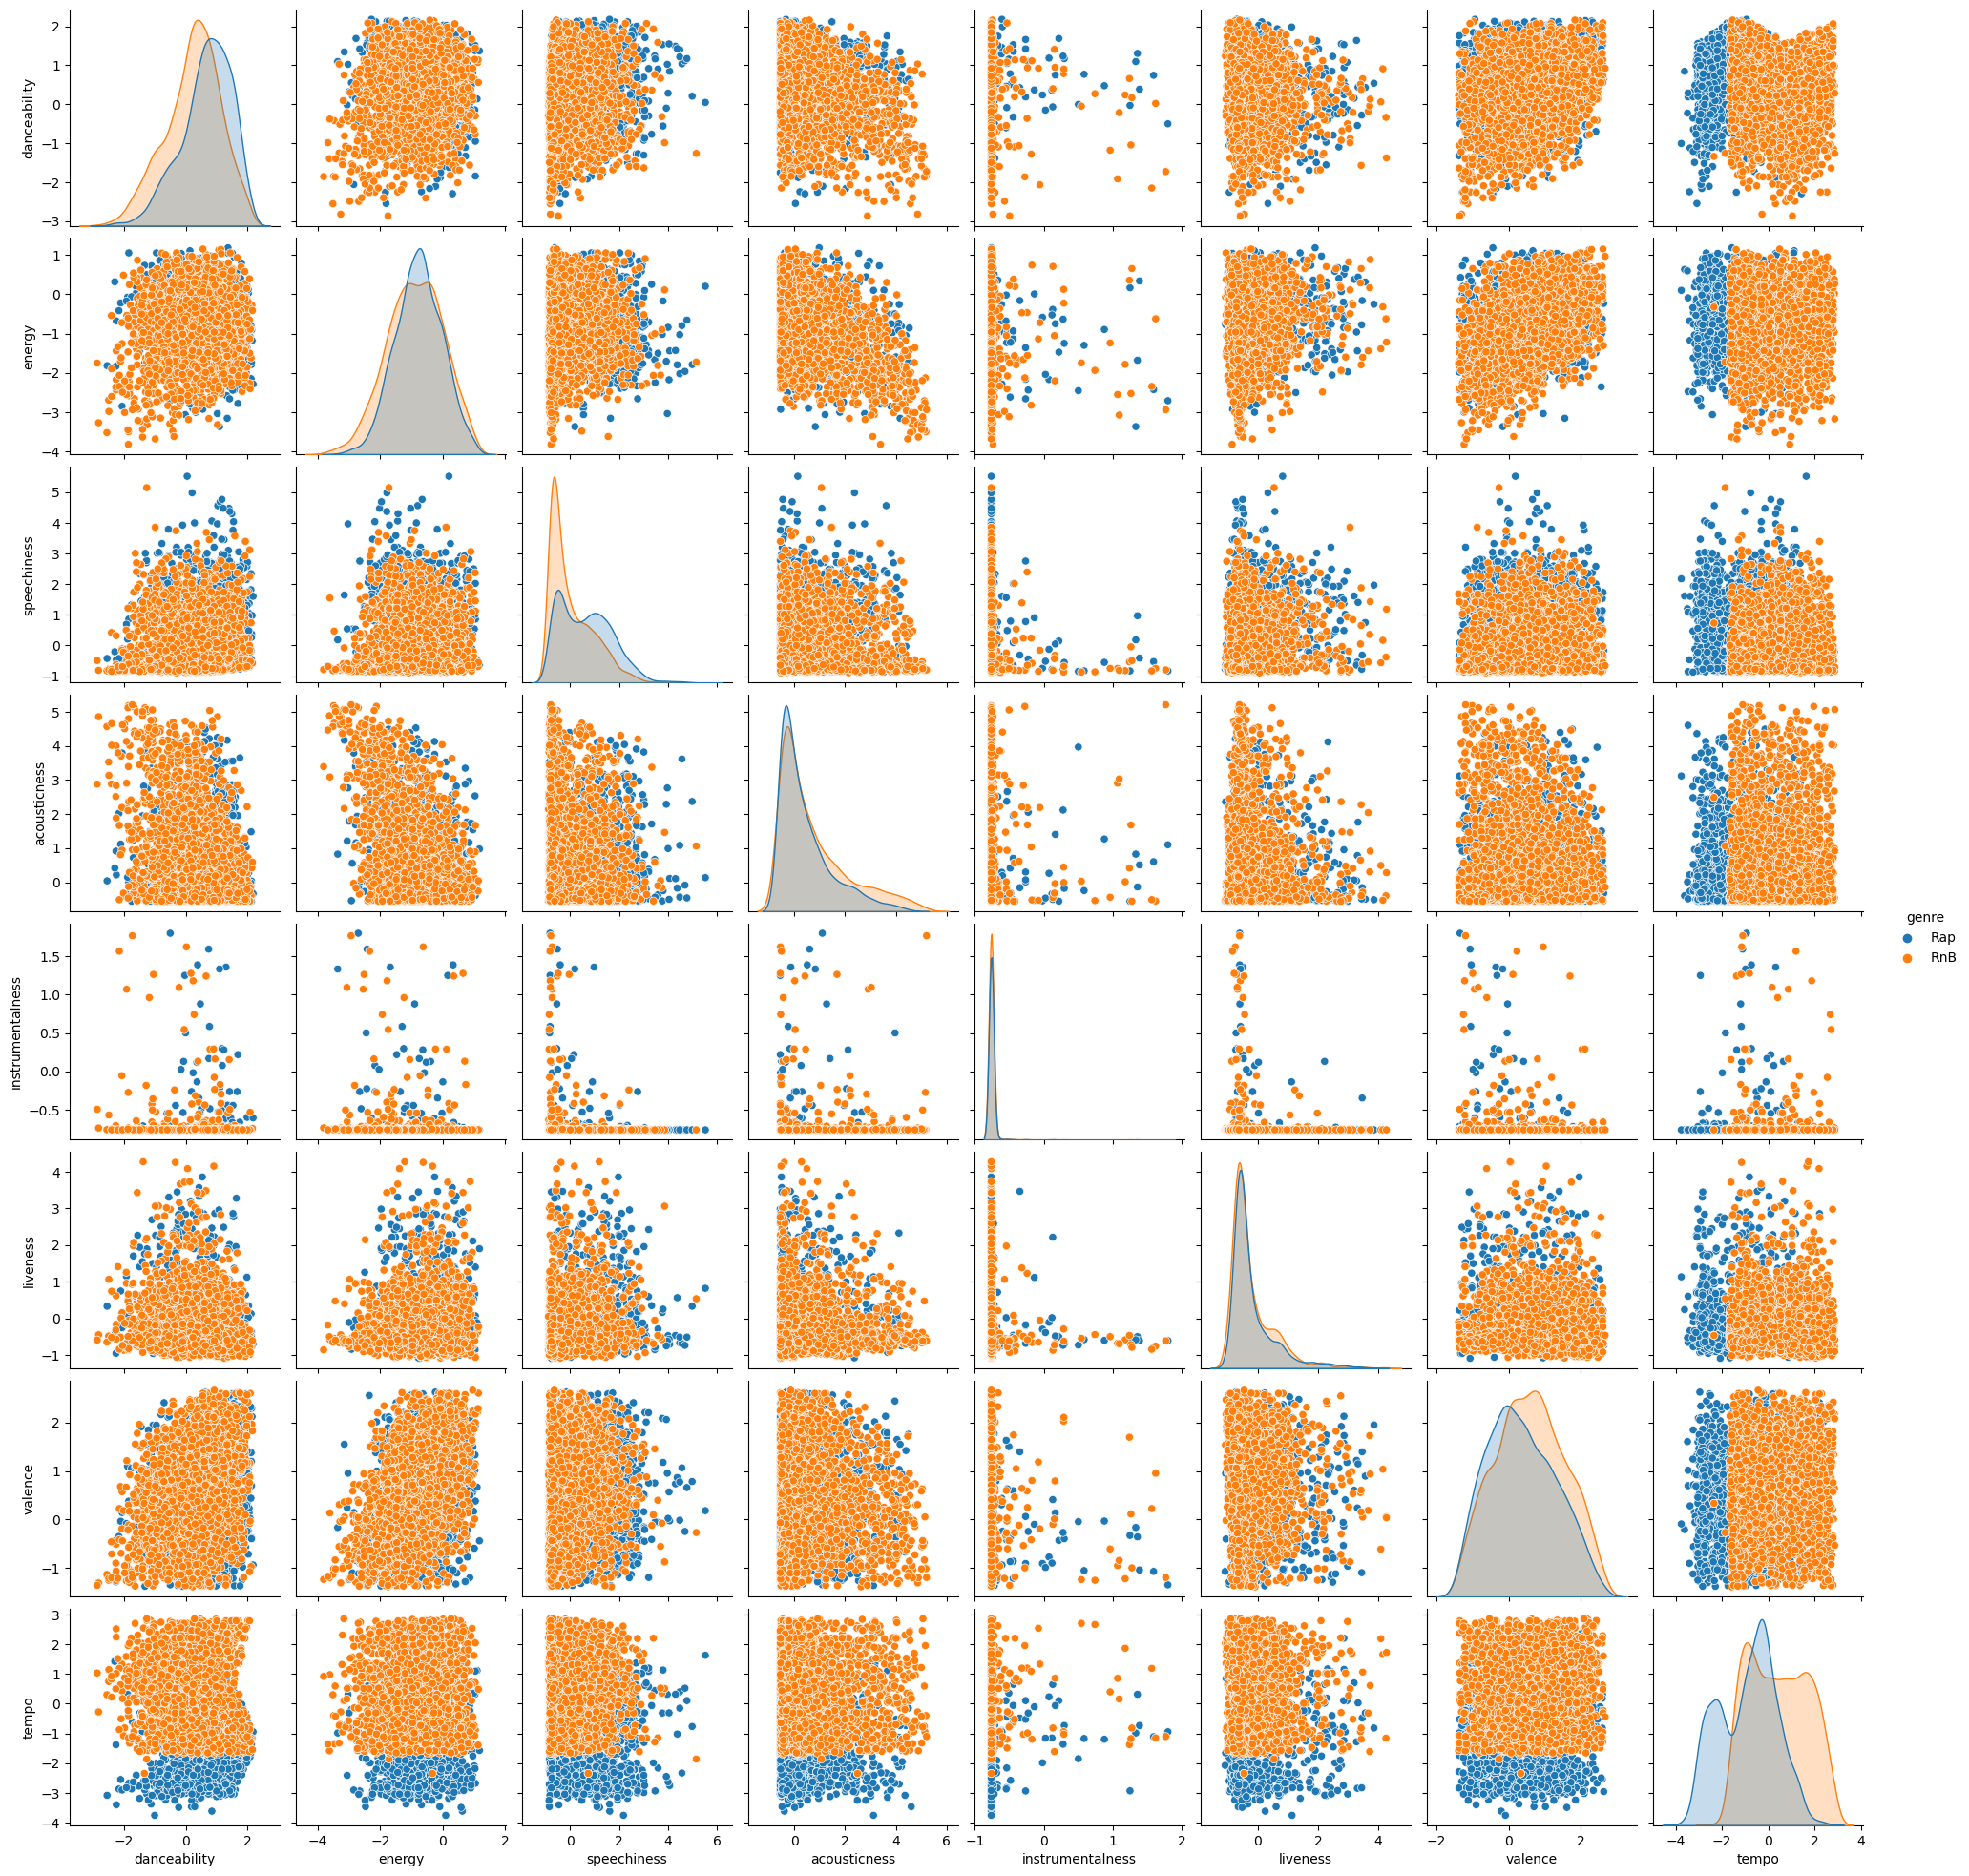
\includegraphics[width=\textwidth]{pairwise-genre-2.png}
        }
    \end{center}
    \caption{Pairwise Scatter Plot: Rap and RnB}
    \label{fig:pairwise-2}
\end{figure}

\subsubsection{Results}
Thus, we run the models using a subset of the data that includes only those records with genre labels "Rap" or "RnB", as well as only the attributes 'tempo' and 'liveliness.' Interestingly, we find that neither K-Means nor DB-Scan was able to make more than one significant cluster out of this subset. Figure \ref{fig:cluster-plot-r2} illustrates this phenomenon. 

 \begin{figure}[!ht]
    \begin{center}
        \resizebox{\columnwidth}{!}{
            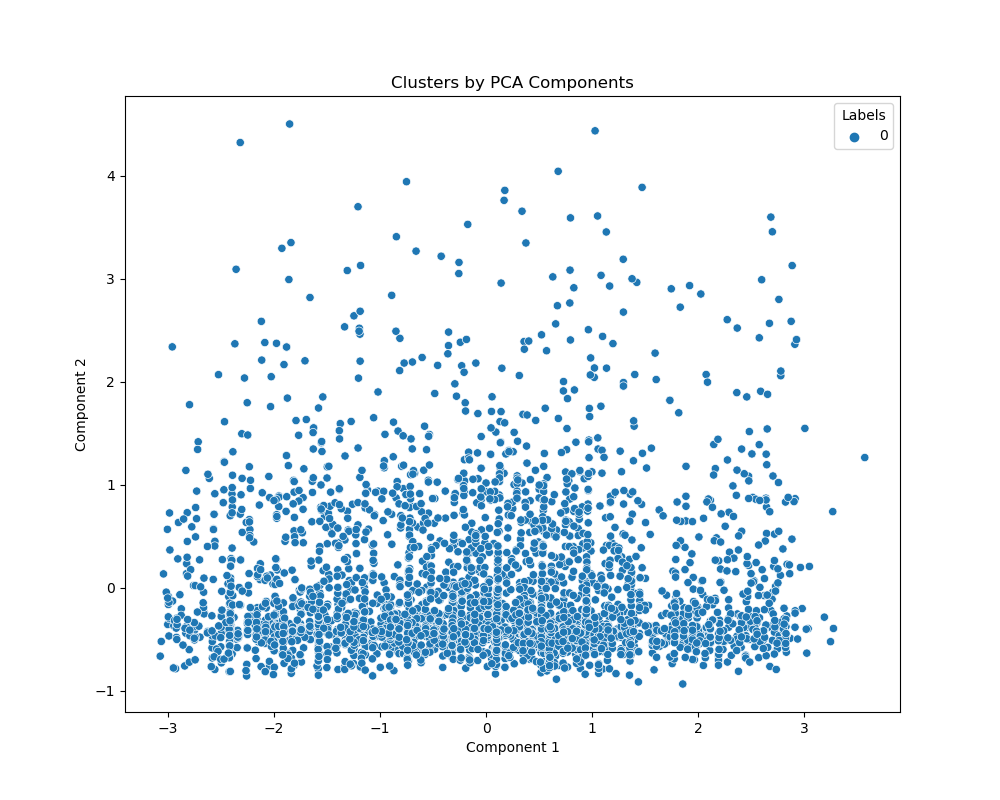
\includegraphics[width=\textwidth]{kmeans-pca-r2.png}
        }
    \end{center}
    \caption{PCA Cluster Plot}
    \label{fig:cluster-plot-r2}
\end{figure}

\subsection{Clustering Tendency}
Our last resort is to determine whether there are actual meaningful clusters to be made from the data. Using the 'hopkins' function from the pyclustertend package, we find the Hopkin's statistic on our training data is 0.14655. Generally, a value of 0.5 or less indicates a lack of meaningful clusters in the data. Because our value is closer to 0, we can observe that indeed this data is not suitable for clustering. Figure \ref{fig:clustering-tendency} is a plot of the data using the first two principal components, with the colors representing genre. We can observe that the data is not spatially distinct, which corroborates the conclusion inferred from Hopkin's statistic.

\begin{figure}[!ht]
    \begin{center}
        \resizebox{\columnwidth}{!}{
            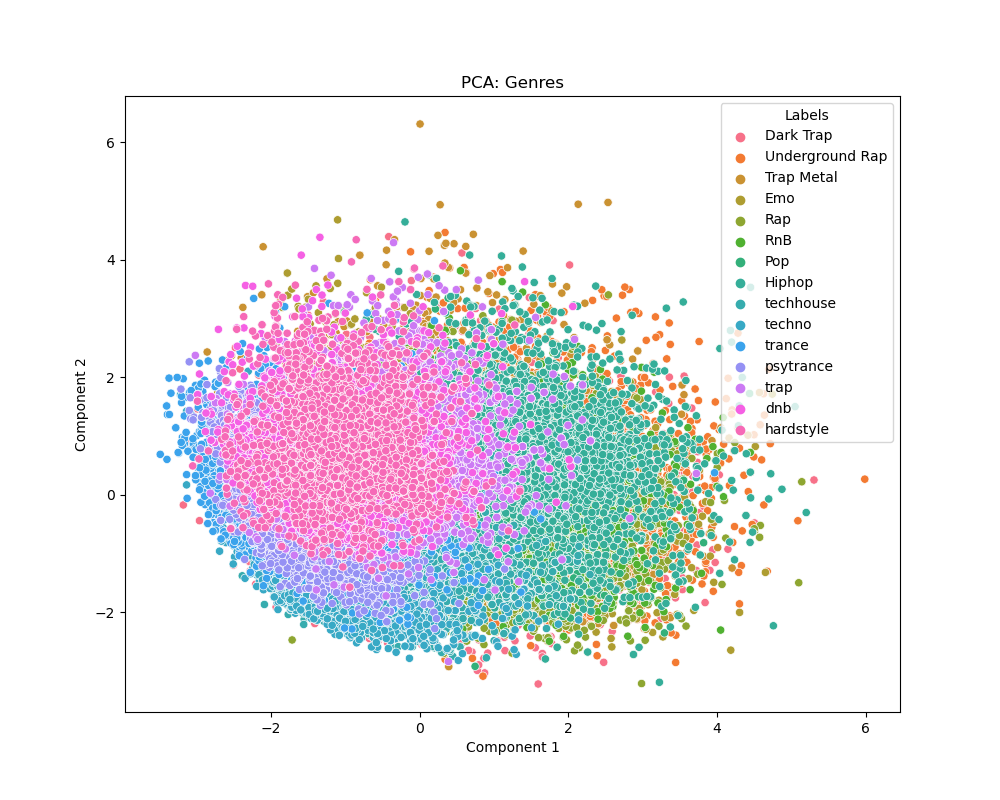
\includegraphics[width=\textwidth]{clustering-tendency.png}
        }
    \end{center}
    \caption{Clustering Tendency}
    \label{fig:clustering-tendency}
\end{figure}



\subsection{Limitations}
There are many limitations to this work. First, we operate under a tight timeline, which may result in implementation or assessment error. This also prohibits us from spending more time discovering why the models aren't working correctly. Furthermore, we did not scrape this data ourselves directly from the API, so there may be hidden errors or bias in the data that are unobservable. It also means we are working with pre-selected genres that may not be a representative sample of Spotify's song database. This is a major limitation because it is likely why the data does not appear to have any statistically significant clusters. 


\section*{VI. Future Work}
There are several possible explanations for the sub-optimal results.  The first would be issues related to data selection. It is possible the dataset we chose was poorly compiled, as evidenced by the imbalance in genres, missing values and low Hopkin's statistic value. This is, in all likelihood, the reason for poor model performance, given that our pre-processing steps were fairly robust. It is also possible that the attributes present in the dataset are simply not conducive for the application we thought of. Solutions for future work then, would involve either choosing a different dataset or using the Spotify API to scrap the data ourselves.  To validate that the data was appropriate for clustering, the Hopkins statistic and pairwise scatterplots need to be \textit{checked first} before proceeding with any pre-processing or modelling. This would prevent us from wasting time trying to cluster data that has no meaningful clusters.

Another possible source of error would be the algorithms used for clustering. Even if the data is clusterable in theory, KMeans and DBScan may be ill suited to this clustering task. One possible explanation for this is because KMeans and DBScan return hard clusters, whereas genre clustering could arguably be seen as more of a soft or fuzzy cluster application. Thus, a more appropriate algorithm for genre clustering might be Automated Fuzzy Clustering, which assigns each sample a probability of belonging to one or more clusters. KMeans and DBScan could possibly still be employed however, given better hyperparameters and a different distance metric. While improved hyperparameter tuning would rely mainly on increased computing power, using a different distance metric that worked better with high-dimensional data could yield much better results. However, more research would need to be conducted in this matter.

Future continuation of this project should thus go through a few changes first.  The first would be selecting more appropriate and balanced data, either using a different dataset or directly working with Spotify API. Then, care should be taken to ensure that the data is indeed clusterable, and does not have any anomalous features or other characteristics that might make clustering difficult. For this the Hopkins statistic, Pearson correlation matrix, scatterplots, and if need be, PCA, should be employed. Lastly, more advanced clustering algorithms (such as Automated Fuzzy Clustering) and more rigorous hyperparameter tuning/distance metric selection should be employed to accurately cluster the data and successfully draw more comprehensive insights.

% \begin{figure}[!ht]
%     \begin{center}
%         \resizebox{\columnwidth}{!}{
%             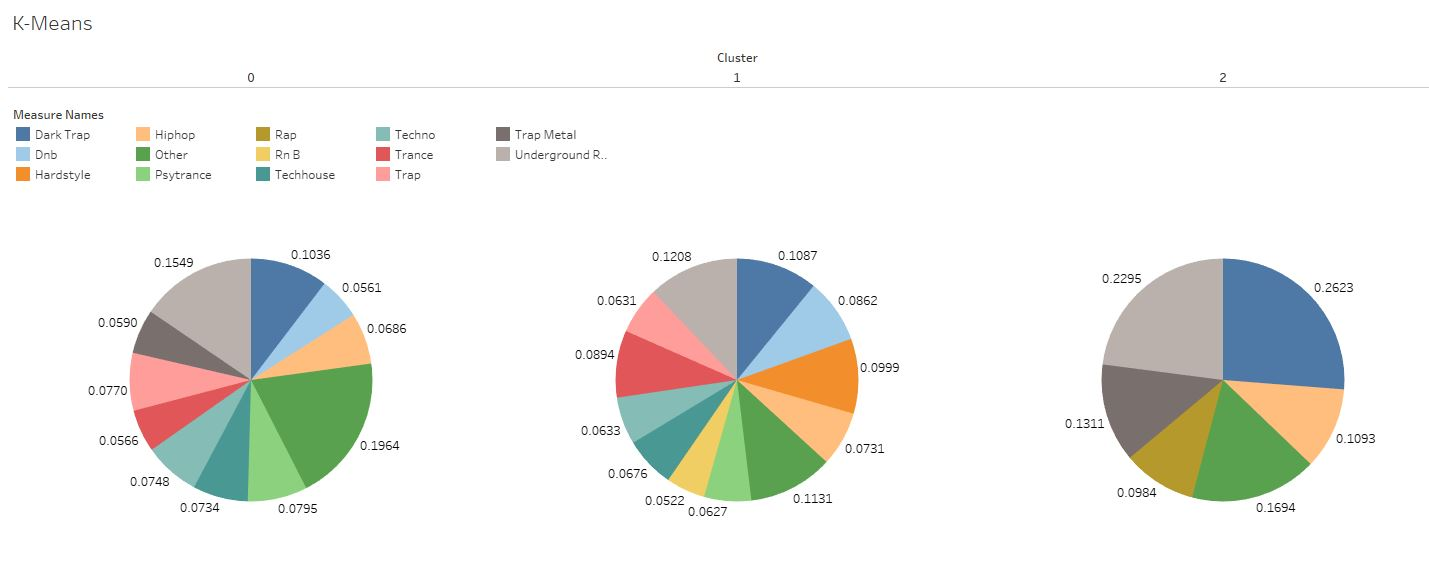
\includegraphics[width=\textwidth]{KMeans Combined.jpg}
%         }
%     \end{center}
%     \caption{Percentage of genres present in each K-Means Cluster}
%     \label{fig:clustering-tendency}
% \end{figure}

% \begin{figure}[!ht]
%     \begin{center}
%         \resizebox{\columnwidth}{!}{
%             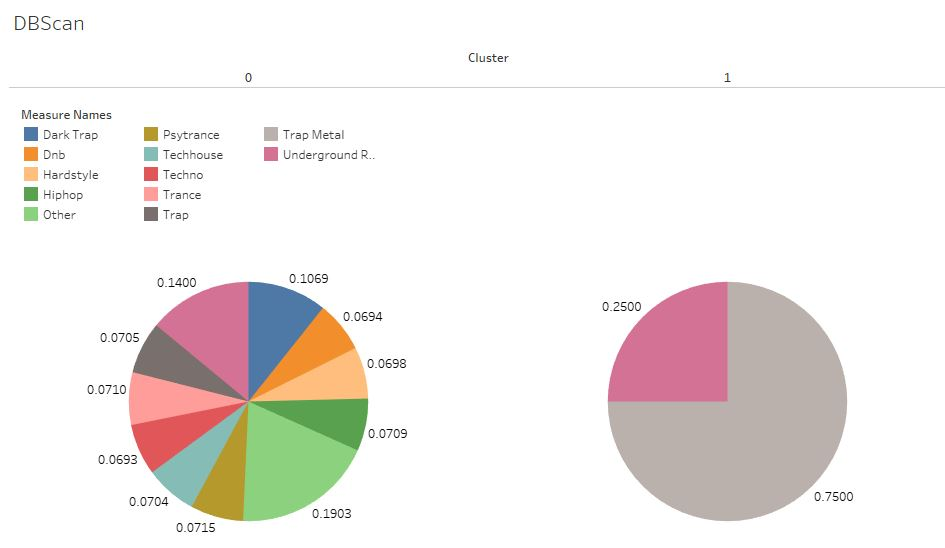
\includegraphics[width=\textwidth]{DBScan Combined.jpg}
%         }
%     \end{center}
%     \caption{Percentage of genres present in each DBScan Cluster}
%     \label{fig:clustering-tendency}
% \end{figure}

\end{document}
